\documentclass{article}
\usepackage{tikz}
\pagestyle{empty}
\begin{document}
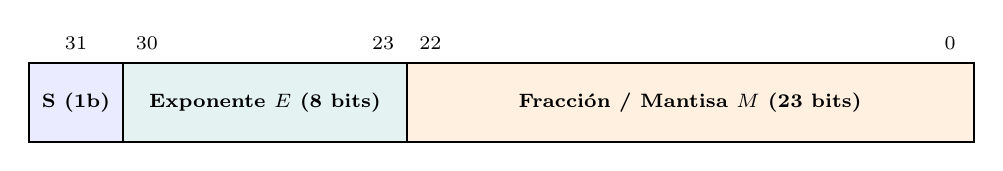
\begin{tikzpicture}

\draw[thick, fill=blue!8] (0,0) rectangle (1.2,1.0) node[pos=.5, font=\scriptsize\bfseries] {S (1b)};
\draw[thick, fill=teal!10] (1.2,0) rectangle (4.8,1.0) node[pos=.5, font=\scriptsize\bfseries] {Exponente $E$ (8 bits)};
\draw[thick, fill=orange!12] (4.8,0) rectangle (12.0,1.0) node[pos=.5, font=\scriptsize\bfseries] {Fracción / Mantisa $M$ (23 bits)};
\node[above, font=\scriptsize] at (0.6,1.05) {31};
\node[above, font=\scriptsize] at (1.5,1.05) {30};
\node[above, font=\scriptsize] at (4.5,1.05) {23};
\node[above, font=\scriptsize] at (5.1,1.05) {22};
\node[above, font=\scriptsize] at (11.7,1.05) {0};

\end{tikzpicture}
\end{document}
